\documentclass[tikz,border=3pt]{standalone}
% Shared preamble for the standalone TikZ diagrams (included after \documentclass).
% Build with build.sh. Language is selected with \def\VI{1} (Vietnamese) or by default English:
%   \LL{English text}{Văn bản tiếng Việt}
\usepackage{fontspec}
\IfFontExistsTF{Times New Roman}{\setmainfont{Times New Roman}}{%
  \setmainfont{times.ttf}[Path=/mnt/c/Windows/Fonts/,
    BoldFont=timesbd.ttf,ItalicFont=timesi.ttf,BoldItalicFont=timesbi.ttf]}
\usepackage{xcolor}
\usepackage{tikz}
\usetikzlibrary{arrows.meta,positioning,calc,fit,backgrounds,patterns,shapes.misc,decorations.pathreplacing}

\newcommand{\LL}[2]{\ifdefined\VI #2\else #1\fi}
\hyphenpenalty=10000 \exhyphenpenalty=10000 \tolerance=9999 \emergencystretch=3em

% --- palette (print-safe: meaning is never carried by colour alone) -----------
\definecolor{ink}{HTML}{1F2937}
\definecolor{muted}{HTML}{6B7280}
\definecolor{rule}{HTML}{9CA3AF}
\definecolor{shfill}{HTML}{DCE8F5}   % shared
\definecolor{shline}{HTML}{2F5D8C}
\definecolor{dedfill}{HTML}{FBE5CF}  % dedicated
\definecolor{dedline}{HTML}{B5651D}
\definecolor{neutral}{HTML}{F3F4F6}
\definecolor{appfill}{HTML}{F6F9FC}
\definecolor{appline}{HTML}{7C93AD}
\definecolor{ctlfill}{HTML}{EFEAF7}
\definecolor{ctlline}{HTML}{6B5B95}
\definecolor{warn}{HTML}{B91C1C}
\definecolor{ta}{HTML}{2A9D8F}       % tenant A
\definecolor{tb}{HTML}{E09F3E}       % tenant B
\definecolor{tc}{HTML}{8E6BBF}       % tenant C
\colorlet{taL}{ta!22}
\colorlet{tbL}{tb!28}
\colorlet{tcL}{tc!24}

\tikzset{
  >=Latex,
  every node/.style={font=\footnotesize, text=ink, inner sep=2pt},
  box/.style={draw=ink!65, rounded corners=1.6pt, line width=0.5pt, fill=white,
              align=center, inner sep=3pt, minimum height=5mm},
  shared/.style={box, fill=shfill, draw=shline},
  ded/.style={box, fill=dedfill, draw=dedline},
  plain/.style={box, fill=neutral, draw=rule},
  ta/.style={box, fill=taL, draw=ta},
  tb/.style={box, fill=tbL, draw=tb},
  tc/.style={box, fill=tcL, draw=tc},
  tenantA/.style={ta}, tenantB/.style={tb}, tenantC/.style={tc},
  zone/.style={draw=appline, fill=appfill, rounded corners=2.5pt, line width=0.6pt},
  ctlzone/.style={draw=ctlline, fill=ctlfill, rounded corners=2.5pt, line width=0.6pt},
  ttl/.style={font=\small\bfseries, text=ink, align=left, inner sep=1pt},
  cp/.style={font=\scriptsize, text=muted, align=center, inner sep=1pt},
  note/.style={font=\scriptsize, text=muted, align=left, inner sep=1pt},
  arr/.style={->, line width=0.6pt, draw=ink!80},
  arrm/.style={->, line width=0.6pt, draw=muted, dashed},
  link/.style={line width=0.5pt, draw=muted},
  bound/.style={line width=0.8pt, draw=warn, dash pattern=on 3pt off 2pt},
  badge/.style={circle, fill=ink, text=white, font=\scriptsize\bfseries, inner sep=1.2pt, minimum size=3.6mm},
}

% a small user glyph (head + shoulders) centred at the given coordinate, colour as 3rd arg

% user glyph: head and shoulders, centred at (x,y); 3rd argument = colour
\newcommand{\user}[3]{%
  \fill[#3] (#1,#2) circle (0.85mm);
  \fill[#3] ($(#1,#2)+(-1.5mm,-2.5mm)$) arc (180:0:1.5mm) -- cycle;}

% Figure: reference model of a multi-tenant architecture (MTA).
% Concepts and their relations only, no technology. Sources: ISO/IEC 17788 (service, customer, user, tenant),
% AWS (2022) control plane vs application plane, Azure Architecture Center (tenant context, tenants vs deployments).
\begin{document}
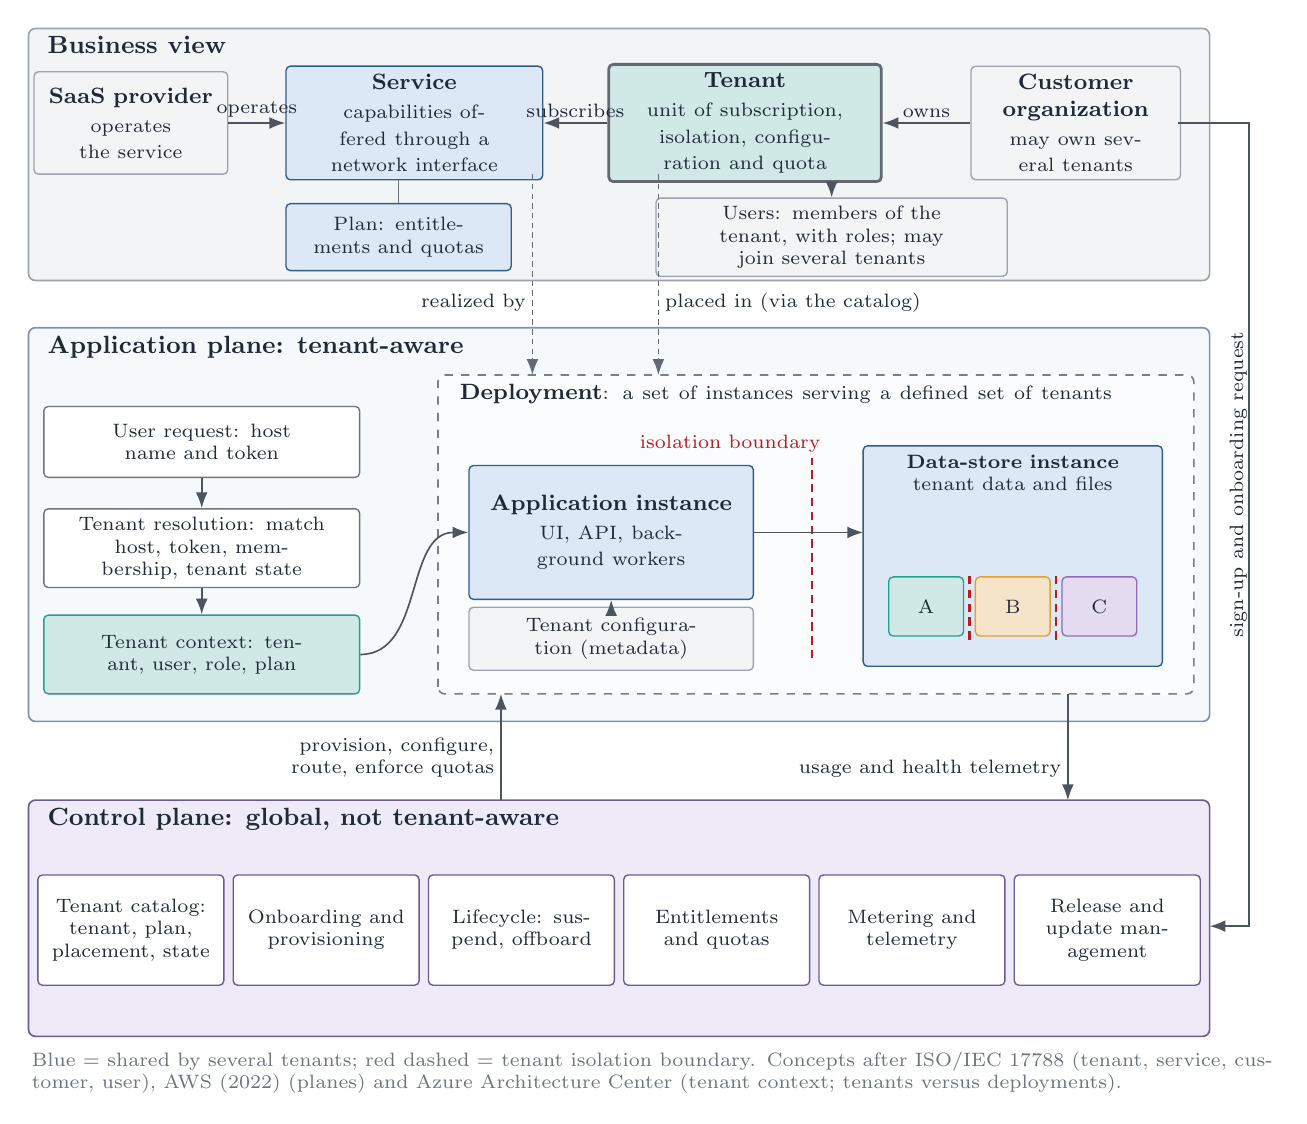
\begin{tikzpicture}[x=1mm,y=1mm]

% ================================================================ business view
\fill[neutral,rounded corners=2.5pt] (0,96) rectangle (150,128);
\draw[rule,rounded corners=2.5pt,line width=0.6pt] (0,96) rectangle (150,128);
\node[ttl,anchor=north west] at (2,127.4) {\LL{Business view}{Góc nhìn nghiệp vụ}};

\node[plain,minimum width=24mm,minimum height=13mm,text width=22.5mm] (prov) at (13,116) {\textbf{\LL{SaaS provider}{Nhà cung cấp SaaS}}\\[1pt]{\scriptsize\LL{operates the service}{vận hành dịch vụ}}};
\node[shared,minimum width=32mm,minimum height=13mm,text width=30.5mm] (serv) at (49,116) {\textbf{\LL{Service}{Dịch vụ}}\\[1pt]{\scriptsize\LL{capabilities offered through a network interface}{các chức năng cung cấp qua giao diện mạng}}};
\node[box,fill=taL,draw=ink!70,line width=1pt,minimum width=34mm,minimum height=13mm,text width=32.5mm] (ten) at (91,116) {\textbf{\LL{Tenant}{Thuê bao}}\\[1pt]{\scriptsize\LL{unit of subscription, isolation, configuration and quota}{đơn vị đăng ký, cô lập, cấu hình và hạn mức}}};
\node[plain,minimum width=26mm,minimum height=13mm,text width=24.5mm] (cust) at (133,116) {\textbf{\LL{Customer organization}{Tổ chức khách hàng}}\\[1pt]{\scriptsize\LL{may own several tenants}{có thể có nhiều thuê bao}}};
\node[shared,minimum width=28mm,minimum height=8.5mm,text width=26.5mm,font=\scriptsize] (plan) at (47,101.5) {\LL{Plan: entitlements and quotas}{Gói: quyền sử dụng và hạn mức}};
\node[plain,minimum width=44mm,minimum height=9mm,text width=42.5mm,font=\scriptsize] (usr) at (102,101.5) {\LL{Users: members of the tenant, with roles; may join several tenants}{Người dùng: thành viên của thuê bao, có vai trò; có thể thuộc nhiều thuê bao}};

\draw[arr] (prov) -- node[above=0.3mm,note,text=ink] {\LL{operates}{vận hành}} (serv);
\draw[arr] (ten) -- node[above=0.3mm,note,text=ink] {\LL{subscribes}{đăng ký}} (serv);
\draw[arr] (cust) -- node[above=0.3mm,note,text=ink] {\LL{owns}{sở hữu}} (ten);
\draw[link] ($(serv.south)+(-2,0)$) -- ($(plan.north)+(0,0)$);
\draw[arr] ($(ten.south)+(11,0)$) -- ($(usr.north)+(0,0)$);

% ================================================================ application plane
\draw[zone] (0,40) rectangle (150,90);
\node[ttl,anchor=north west] at (2,89.4) {\LL{Application plane: tenant-aware}{Mặt phẳng ứng dụng: nhận biết thuê bao}};

% access path (left column)
\node[box,minimum width=40mm,minimum height=9mm,text width=38mm,font=\scriptsize] (rq) at (22,75.5) {\LL{User request: host name and token}{Yêu cầu người dùng: tên miền và mã xác thực}};
\node[box,minimum width=40mm,minimum height=10mm,text width=38mm,font=\scriptsize] (res) at (22,62) {\LL{Tenant resolution: match host, token, membership, tenant state}{Nhận diện thuê bao: đối chiếu tên miền, mã xác thực, tư cách thành viên, trạng thái thuê bao}};
\node[box,fill=taL,draw=ta,minimum width=40mm,minimum height=10mm,text width=38mm,font=\scriptsize] (ctx) at (22,48.5) {\LL{Tenant context: tenant, user, role, plan}{Ngữ cảnh thuê bao: thuê bao, người dùng, vai trò, gói}};
\draw[arr] (rq) -- (res);
\draw[arr] (res) -- (ctx);

% deployment frame
\draw[dashed,draw=ink!60,line width=0.6pt,rounded corners=2.5pt,fill=white,fill opacity=0.55] (52,43.5) rectangle (148,84);
\node[font=\footnotesize\bfseries,anchor=north west,text width=94mm] at (54,83.6) {\LL{Deployment}{Bản triển khai}{\scriptsize\mdseries\LL{: a set of instances serving a defined set of tenants}{: tập các thể hiện phục vụ một nhóm thuê bao xác định}}};
\node[shared,minimum width=36mm,minimum height=17mm,text width=34mm] (app) at (74,64) {\textbf{\LL{Application instance}{Thể hiện ứng dụng}}\\[1pt]{\scriptsize\LL{UI, API, background workers}{giao diện, API, tiến trình nền}}};
\node[plain,minimum width=36mm,minimum height=8mm,text width=34mm,font=\scriptsize] (cfg) at (74,50.5) {\LL{Tenant configuration (metadata)}{Cấu hình thuê bao (siêu dữ liệu)}};
\draw[arr] (cfg) -- (app);
\draw[arr] (ctx.east) to[out=0,in=180] (app.west);
\draw[bound] (99.5,48) -- (99.5,73.4);
\node[note,text=warn,anchor=south east,text width=24mm,align=right] at (101,73.8) {\LL{isolation boundary}{ranh giới cô lập}};
\node[shared,minimum width=38mm,minimum height=28mm] (dat) at (125,61) {};
\node[font=\scriptsize,text width=36mm,align=center] at (125,71.6) {\textbf{\LL{Data-store instance}{Thể hiện kho dữ liệu}}\\\LL{tenant data and files}{dữ liệu và tệp của thuê bao}};
\foreach \x/\c/\n in {114/ta/A,125/tb/B,136/tc/C} { \node[\c,minimum width=9.5mm,minimum height=7.5mm,font=\scriptsize] at (\x,54.6) {\n}; }
\draw[bound] (119.5,50.4) -- (119.5,58.8);
\draw[bound] (130.5,50.4) -- (130.5,58.8);
\draw[arr] (app.east) -- (99.5,64) -- (106,64);

% ================================================================ control plane
\draw[ctlzone] (0,0) rectangle (150,30);
\node[ttl,anchor=north west] at (2,29.4) {\LL{Control plane: global, not tenant-aware}{Mặt phẳng điều khiển: dùng chung toàn hệ thống, không nhận biết thuê bao}};
\foreach \i/\en/\vi in {
  0/{Tenant catalog: tenant, plan, placement, state}/{Danh mục thuê bao: thuê bao, gói, vị trí, trạng thái},
  1/{Onboarding and provisioning}/{Đăng ký và cấp phát tài nguyên},
  2/{Lifecycle: suspend, offboard}/{Vòng đời: tạm ngưng, chấm dứt},
  3/{Entitlements and quotas}/{Quyền sử dụng và hạn mức},
  4/{Metering and telemetry}/{Đo lường và giám sát},
  5/{Release and update management}/{Quản lý phát hành và cập nhật}} {
  \node[box,fill=white,draw=ctlline,minimum width=23mm,minimum height=14mm,text width=21.5mm,font=\scriptsize] at (13+\i*24.8,13.5) {\LL{\en}{\vi}};
}

% ================================================================ relations across bands
\draw[arr,draw=ink!70,dash pattern=on 2pt off 1.5pt] (64,109.5) -- node[left=0.4mm,note,text=ink,pos=0.64] {\LL{realized by}{hiện thực bởi}} (64,84);
\draw[arr,draw=ink!70,dash pattern=on 2pt off 1.5pt] (80,109.5) -- node[right=0.4mm,note,text=ink,pos=0.64] {\LL{placed in (via the catalog)}{được đặt vào (qua danh mục)}} (80,84);
\draw[arr] (60,30) -- node[left=0.4mm,note,text=ink,text width=50mm,align=right,pos=0.4] {\LL{provision, configure, route, enforce quotas}{cấp phát, cấu hình, định tuyến, áp hạn mức}} (60,43.5);
\draw[arr] (132,43.5) -- node[left=0.4mm,note,text=ink,text width=36mm,align=right,pos=0.7] {\LL{usage and health telemetry}{số liệu sử dụng và tình trạng}} (132,30);
\draw[arr] (146,116) -- (155,116) -- node[right=0.2mm,note,text=ink,rotate=90,anchor=south,pos=0.45] {\LL{sign-up and onboarding request}{yêu cầu đăng ký và cấp phát}} (155,14) -- (150,14);

\node[note,anchor=north west,text width=158mm] at (0,-1.5) {\LL{Blue = shared by several tenants; red dashed = tenant isolation boundary. Concepts after ISO/IEC 17788 (tenant, service, customer, user), AWS (2022) (planes) and Azure Architecture Center (tenant context; tenants versus deployments).}{Xanh dương = dùng chung nhiều thuê bao; đứt nét đỏ = ranh giới cô lập thuê bao. Khái niệm theo ISO/IEC 17788 (thuê bao, dịch vụ, khách hàng, người dùng), AWS (2022) (các mặt phẳng) và Azure Architecture Center (ngữ cảnh thuê bao; thuê bao so với triển khai).}};

\end{tikzpicture}
\end{document}
